% high
% for MEDEA CAN printing
%
\documentclass[10pt,twocolumn,dvips]{article}
\usepackage[english]{babel}
\usepackage{epsfig}
%
%
% official IEEE double column format
\textwidth 6.5in
\textheight 8.875in
\topmargin -0.6in
%
%
% some publishers want no page numbers for final print
\pagestyle{empty}
%
%
\begin{document}
%
\title{Realizing High IPC Through a Scalable Memory-Latency Tolerant
Multipath Microarchitecture}
%
\author{
D. Morano, A. Khalafi, D.R. Kaeli\\
Northeastern University\\
{dmorano, akhalafi, kaeli}@ece.neu.edu\\
\and
A.K. Uht \\
University of Rhode Island\\ 
uht@ele.uri.edu
}
%
% no date for CAN printing
\date{}
%
\maketitle
%
%
% uncomment the following for page with no page numbers (for IEEE)
\thispagestyle{empty}
%
%
\begin{abstract}
A microarchitecture is described that achieves high performance on
conventional single-threaded program codes without compiler
assistance.  To obtain high instructions per clock (IPC) for inherently
sequential (e.g., SpecInt-2000 programs), a large number of
instructions must be in flight simultaneously.  However, several
problems are associated with such microarchitectures, including
scalability, issues related to control flow, and memory latency.

Our design investigates how to utilize a large mesh of processing
elements in order to execute a single-threaded program.  
We present a basic overview of our microarchitecture and discuss how it
addresses scalability as we attempt to execute many instructions in
parallel.  
The microarchitecture makes use of control and value speculative
execution, multipath execution, and a high degree of out-of-order execution
to help extract instruction level parallelism.
Execution-time
predication and time-tags for operands 
are used for maintaining program order.
We provide
simulation results for several geometries of our microarchitecture
illustrating a range of design tradeoffs.  
Results are also presented that show the small performance
impact over a range of memory system latencies.
\end{abstract}
%
%
\section{Introduction}
%
A number of studies into the limits of instruction level 
parallelism (ILP) have
been promising in that they have shown that there is 
a significant amount of parallelism within
typical sequentially oriented single-threaded programs
(e.g., SpecInt-2000).  
The work of 
Lam and Wilson ~\cite{Lam92},
Uht and Sindagi ~\cite{Uht95},
Gonzalez and Gonzalez ~\cite{Gon97}
have shown that there exists a great amount of instruction level
parallelism (ILP) that is not being exploited by any existing
computer designs.
Unfortunately, most of the fine-grained ILP
inherent in integer sequential programs
spans several basic blocks.  
Data and control independent instructions, that may exist
far ahead in the program instruction stream, need to be
speculatively executed to exploit all possible inherent ILP.

A large number of instructions need to be fetched
each cycle and executed concurrently in order to achieve this.
We need to find the available program ILP at runtime and to 
provide sufficient hardware to expose, schedule,
and otherwise manage the out-of-order speculative execution of
control independent instructions.
Of course, the microarchitecture has to also provide a means
to maintain the architectural program order that
is required for proper program execution.

We present a novel microarchitecture in this paper that can
be applied to any existing ISA.  Our microarchitecture
is targeted at obtaining
substantial program speedups on integer codes.
The microarchitecture can speculatively execute hundreds
of instructions ahead in the program instruction stream and
thus expose large amounts of inherent ILP.
We use multipath execution to cover latencies associated
with branch mispredictions.
We also take advantage of control
and data independent instructions through our use of
execution-time predication.
Since we provide local buffering (a form of {\em L0 caching}) throughout 
our grid layout, we can satisfy a large number of accesses without
accessing higher levels of the memory hierarchy.  Further, since 
our design utilizes a form of value speculation on all operands, we consume 
the present value of a register, even if an outstanding load is pending
which targets this register.
%
\subsection{Related Work}
%
There have been several attempts at substantially increasing
program IPC through the exploitation of ILP.
The Multiscalar processor architecture \cite{Soh95}
attempted 
to realize substantial IPC speedups over conventional superscalar
processors.  However, the approach is quite different than ours 
in that Multiscalar relies on compiler participation where we do not.
A notable attempt at realizing high IPC was done by
Lipasti and Shen on their Superspeculative
architecture~\cite{Lip97}.  They achieved an IPC of
about 7 with realistic hardware assumptions.
The Ultrascalar machine~\cite{Hen00}
achieves {\em asymptotic} scalability,
but only realizes a small amount of IPC due to its 
conservative execution model.
Nagarajan et al proposed a {\em Grid Architecture} of ALUs
connected by an operand network~\cite{Nag01}.  
This has some similarities to our work.
However, unlike our work, their microarchitecture
relies on the coordinated use of the compiler along with
a new ISA to obtain higher IPCs.

The rest of this paper is organized as follows.
Section 2 reviews the critical elements
of our proposed microarchitecture.
Section 3 presents simulation results for a range of
machine configurations, and shows the potential
impact of multipath execution when applied.
We also discuss how our microarchitecture reduces
our dependence on the memory system by providing a large
amount of local caching on our datapath. 
We summarize and conclude in section 4.
%
%
\section{The Microarchitecture}
%
We have described most of the details of this microarchitecture
in~\cite{EPAR}.   We will review these details at a level to allow
the reader to grasp a general understanding as it applies to the
memory system performance. 
In addition, this paper presents a microarchitecture with a realistic 
memory subsystem and we therefor are better able to
evaluate the performance impact of the memory hierarchy.

The microarchitecture is very aggressive in terms of
the amount of speculative execution it performs.
This is realized through a large amount of scalable execution
resources.
Resource scalability
of the microarchitecture is achieved through its distributed nature
along with repeater-like components that limit the maximum bus
spans.
Contention for major centralized structures is avoided.
Conventional centralized resources like a register file,
reorder buffer, and centralized execution units, are eliminated.

The microarchitecture also 
addresses several issues associated with conditional branches.
Spawning alternative speculative paths when encountering conditional
branches is done to avoid branch misprediction penalties.
Exploitation of control
and data independent instructions beyond the join of a 
hammock branch ~\cite{Fer87,Uht86}
is also capitalized upon where possible.
Choosing which paths in multipath execution should
be given priority for machine resources is also addressed
by the machine.
The predicted program path is referred to as the {\em mainline} path.  
We give execution resource priority to this mainline path with respect
to any possible alternative paths.
Since alternative paths have lower priority with
respect to the mainline path, they are referred
to as {\em disjoint} paths.  
This sort of strategy for the spawning of disjoint 
paths results in what is termed {\em disjoint eager execution} (DEE).
We therefore refer to disjoint paths as simply {\em DEE paths}.
These terms are taken from Uht~\cite{Uht95}.

Time-tags are the basic mechanism
used in the microarchitecture to order all operands, including
memory operands, while they are being used by instructions
currently being executed.  Time-tags are small values that
are associated with operands that serve as both an identifying
tag and as a means to order them with respect to each other.
The Warp Engine~\cite{Cle95}
also used time-tags to manage large amounts of speculative execution,
but our use of them is much simpler than theirs.
Time-tags are present on some recent machines (e.g., P6, Pentium 4),
though are used for different purposes than as 
employed in our microarchitecture.   
%
%
\subsection{Microarchitecture Components}
%
Figure~\ref{fig:high} provides a high-level view of our microarchitecture.
%
\begin{figure}
\centering
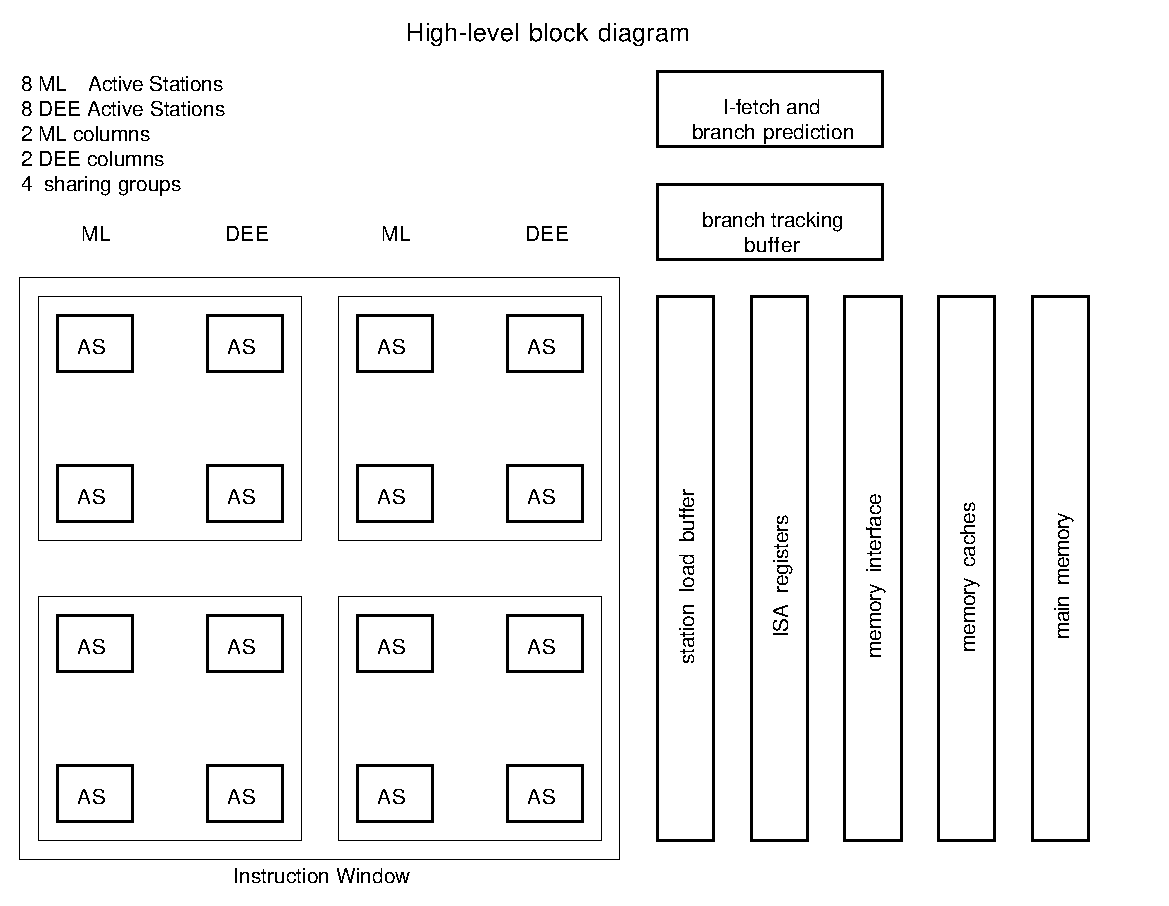
\epsfig{file=high.eps,width=3.24in}
\caption{{\em High-level View of the Distributed Microarchitecture.} 
Shown are the major hardware components of the microarchitecture.
With the exception of the 
execution window block, this is similar to most conventional
microarchitectures}.
\label{fig:high}
\end{figure}
%
Our microarchitecture shares many basic 
similarities to most conventional
machines.
The main memory block,
the L2 cache (unified in the present case), and the L1 instruction 
cache are all rather similar to those in common use.
Except for the fact that the main memory, L2 cache, and L1 data
cache are all address-interleaved, there is nothing further
unique about these components. 
Our L1 data cache is similar to
most conventional data caches except that it also has the ability to
track speculative memory writes using a store buffer.
Our L1 d-cache shares a similar goal with the 
Speculative Versioning Cache \cite{Gop98} 
but is simpler in some respects.
Since we allow speculative memory writes to propagate
out to the L1 data cache, multiple copies
of a speculative write may be present in the L1 data cache store buffer 
at any time.  They are differentiated from each other
through the use of time-tags.  

The i-fetch unit first fetches instructions from i-cache
along one or more predicted program paths.
Due to our relatively large instruction fetch bandwidth
requirement, we allow for the fetching of up to two i-cache
lines in a single clock.
Instructions are immediately
decoded after being fetched.
All further handling of the instructions is done in their decoded
form.
Decoded instructions are then staged
into an {\em instruction dispatch buffer}
so that they are available to be dispatched
into the {\em execution window} when needed.  
The execution window is where
our microarchitecture differs substantially from existing machines.
This instruction dispatch buffer is organized so that
a large number of instructions can be broadside loaded into the
execution window in a single clock.
The multiple buses going from the i-fetch unit to the
execution window in Figure \ref{fig:high} are meant to
reflect this operation.  
The maximum number of instructions dispatched into the
execution window at a time (in a single clock) is termed
the {\em column height} of the machine.  
%
%
\subsection{The Execution Window}
%
Figure \ref{fig:window} shows a more detailed view
of the execution window with its subcomponents.
%
\begin{figure}
%\vspace{0.2 in}
%\setlength{\epsfxsize}{10cm}%7
%\centerline{\epsfbox{window.eps}}
\centering
\epsfig{file=window.eps,width=3.24in}
\caption{{\em The Execution Window.} 
Shown is a layout of the Active Stations (AS) and Processing Elements (PE)
along with some bus interconnections to implement a large,
distributed microarchitecture. Groups of ASes share a PE; a group is called
a {\em sharing group}.}
\label{fig:window}
\end{figure}
%
We have extended the idea of the reservation
station \cite{Tom67} to provide the basic building block for a distributed
microarchitecture.  
In our microarchitecture,
an output result is not looped back to the input of the same reservation
station
that provided the result but rather is forwarded to different
stations that are spatially separated, in silicon or circuit board space,
from the first.  
This operation is termed {\em operand forwarding}.
Our adaptation of the
reservation station is termed an {\em active station} (AS).
Like a reservation station (or an {\em issue slot} for machines
that have an issue window), an AS can only hold a single
instruction at a time.  
However, instructions may be issued from the AS to its associated execution 
unit multiple times rather than only once.  
Several ASes may share the use of one or more execution units.
The execution units that are dispersed among the ASes are termed
{\em processing elements} (PEs).  Each PE 
may consist of an unified all-purpose execution unit capable of
executing any of the possible machine instructions or, more likely,
consist of
several functionally clustered units
for specific classes of instructions (integer ALU, FP, or other).
Instructions execute
speculatively without necessarily waiting for their correct
operands to arrive.  Re-executions of instructions occur as needed
to guarantee proper program dependencies.
An instruction remains in the AS, possibly executing many times,
until it can be retired (either committed or squashed).

As part of the strategy to allow for a scalable microarchitecture,
we lay the ASes out in silicon on
a two-dimensional grid whereby sequentially
dispatched instructions will go to sequential ASes down a column of
the two-dimensional grid of ASes.  
The use of a two-dimensional
grid simply allows for a design implementation
in either a single silicon IC or through several
suitable ICs on a multi-chip module.
The number of ASes in the height dimension of the grid is the
same as the column height of the machine, introduced previously.
The example machine of Figure~\ref{fig:window} has a column height of
six (six instruction load buses shown feeding six ASes). 

Groups of active stations, along with their associated PE,
are called a {\em sharing group} (SG), since they {\em share}  
execution resources with the set of ASes in the group.
The example machine of Figure~\ref{fig:window}
consists of two columns of SGs, each with two SG rows.
Sharing groups somewhat resemble
the relationship between the register file, reorder buffer,
reservation stations, and function units of most conventional
microarchitectures.  They have a relatively high degree of bus
interconnectivity amongst them, as conventional microarchitectures do.
The ASes serve the role of both the
reservation station and the reorder buffer of more conventional
machines.
The transfer of a decoded instruction, along with its associated operands,
from an AS to its PE is isolated to within the SG they belong to.
The use of this execution resource sharing arrangement also allows
for reduced interconnections between adjacent SGs.
Basically, only operand results need to flow from one SG
to subsequent ones.

In our present microarchitecture, we always have two 
columns of ASes within a SG.
The first AS-column is
reserved for the mainline
path of the program and is
labeled {\em ML} in the figure.
The second column of ASes is reserved for the possible
execution of a DEE path and is labeled {\em DEE} in the figure.

In this machine example, each SG contains three rows of ASes
(for a total of six) and a single PE.
Many machine sizes have been explored so far but only a subset
of these sizes is further investigated in this paper.
A particular machine is generally characterized using the 4-tuple: 
%
\begin{itemize}
\item{sharing group rows}
\vspace{-0.10in}
\item{active station rows per sharing group}
\vspace{-0.10in}
\item{sharing group columns}
\vspace{-0.10in}
\item{number of DEE paths allowed}
\end{itemize}   
%
These four characteristic parameters of a given machine
are greatly influential to its performance, as expected,
and the 4-tuple is termed the {\em geometry} 
of the machine.
These four numbers are usually concatenated
so that the geometry of the machine in Figure \ref{fig:window}
would be abbreviated {\em 2-3-2-2}.

When an entire column
of ASes is free to accept new instructions, generally
an entire column worth of instructions are dispatched in a single
clock to the free AS-column 
from the instruction dispatch buffer.
Conditional branches are
predicted just before they are entered into the instruction
dispatch buffer.
The prediction of a branch then accompanies the decoded instruction
if and when it might be dispatched.

Also employed within the execution window is a scheme to
dynamically predicate, at execution time, 
all instructions that have been dispatched
into active stations.  
This predication scheme essentially provides for each dispatched
instruction (now in an AS)
an {\em execution predicate}.  
These execution predicates are just a single bit, 
but are entirely maintained and manipulated within the microarchitecture
itself, not being visible at the ISA level of abstraction.

From actual VHDL implementation and synthesis of 
the described machine components, and using the technology design rules used
in the EV8 microprocessor \cite{Preston02},
an estimate of the size of a machine in silicon can be made.
It is estimated that an 8-4-8-8 geometry could be implemented
in about 600 million transistors.  
When just considering the
execution window of the machine (Figure \ref{fig:window}),
most of the silicon space (as
might be expected) is taken up by execution resources,
labeled as {\em PEs}, with floating point execution being particularly
large.  
Components, such as the ASs, are relatively small.  
The amount of cache in the MFUs is flexible and
usually takes up the next most amount of space after the execution units.  
A variety of larger sized machines could be implemented
in silicon (as transistor budget allows) or in multichip modules.
%
%
\subsection{Operand Forwarding and Machine Scalability}
%
An interconnect fabric is provided to forward result
operands from earlier ASes (in program ordered time) to 
later ASes.  
Result operands are one of three possible types: register, memory, and
instruction execution predicates.
The interconnect allows for arbitrary numbers of sharing
groups to be used in a machine while still keeping all bus
spans to a fixed (constant) length.
All of the buses in
Figure \ref{fig:window}, with the exception of the instruction
load buses, form the interconnection fabric.
Several bus arrangements are possible but we only
further explore one such arrangement (that shown in the figure).
In the general case, several buses are used in parallel to make up
a single forwarding span.
This is indicated by the use of the
bold lines for buses in the figure.
More than one
bus in parallel for each bus span is generally required to meet
the operand forwarding bandwidth needs of the machine.

Active bus repeater components are used (and required) to 
allow for constant length bus spans.
A bus repeater component is generally termed a
{\em forwarding unit} (FU) and is so labeled in the figure.
These forwarding units do more than just repeat operand values from
one span of a bus to the next.
For registers and memory, operands are filtered so that
redundant forwards of the same value (as compared with that last forwarded)
are eliminated.  These can also be termed {\em silent forwards}.
This filtering provides a means to reduce the overall bandwidth
requirements of the forwarding interconnection fabric.
Each forwarding unit employed in the present work also has a small
amount of storage for memory operands.
This storage serves as a cache for memory operand values.
We term this small cache storage a {\em L0 data cache}.
In the present design, the L0 data cache is fully associative,
containing 32 entries, and resides within the memory filtering
unit.  There is one memory filtering unit per column in the
models evaluated in this paper.  We also include data that is
{\em snarfed}~\footnote{Snarfing implies we snoop a bus, find a
match on the current bus contents, and we read the associated
data value.}
off the bus on a bus snoop and L0 data cache hit.
The entire bus structure serves as a local caching network.

For register and predicate operands, values that are generated
by ASes contend for one of the outbound buses
(labeled {\em shared operand forwarding buses} in the figure) 
to forward the value.
Requests for bus use will be satisfied with any bus clock-slot that may be
available on any of the buses in parallel, belonging to
a given span.  All other ASes on the outbound bus span snoop
operand values forwarded from previous (in program order)
ASes.  In addition, a forwarding unit (the bus repeater) also
snoops the same operands and forwards the operand value to the
next bus span if necessary (if the value was different than the previous
value).  For register and predicate operands, they are also
looped around from the bottom of one column of SGs
to the top of the next column of SGs.  
Operands from the bottom of the
far right column of SGs gets looped around to the
top of the far left column. Memory operands also utilize the
same loop structure. 
This behavior forms the characteristic ring pattern of operand flow,
inherent in many microarchitectures \cite{Ranganathan98}.
Forming a closed loop
with these buses, and essentially just renaming columns (identifying the
one closest to retirement), is easier than physically transferring
(shifting) the contents of one column to the next when a column
of ASes retires.

For memory operands, a second operand forwarding strategy is used.
When memory operands are generated by ASes, the AS contends
for one of the outbound buses 
(labeled {\em shared operand forwarding buses} in Figure~\ref{fig:window}) 
in order to forward the operand value.
However, unlike the register and predicate operand forwarding
strategy, a memory load requests (without data)
travels backwards, in program ordered
time, and gets snooped by the forwarding units that are at the top
of each SG column.  This is done so that the operand can
be transferred onto a {\em memory operand transfer bus}, shown
at the top of Figure \ref{fig:window}.  
These buses are address-interleaved and
provide the connectivity to transfer memory operands (generally
speculative) to the L1 data cache.
Memory values are tentatively stored in a store buffer, along with 
their associated operand
time-tags, until a committed value is determined.
Similarly, operands returning from the L1 data cache to service requests
from ASes are first put on one of the memory operand transfer buses (based
on the interleave address of the operand).  These operands then get snooped
by all of the forwarding units at the top of each SG
column, after which the operand is forwarded on a shared operand
forwarding bus (shown vertically) to reach the requesting ASes.

Persistent register, predicate state and some persistent
memory state is stored in the forwarding units.
Persistent state is not stored indefinitely in any single forwarding
unit but is rather stored in different units as the machine
executes column shift operations (columns of ASes get retired
and committed).  However, this is all quite invisible to the ISA.
This microarchitecture also implements precise exceptions~\cite{Smi88}
similarly to how they
are handled in most speculative machines.  
A speculative exception (whether on the mainline path or a DEE path)
is held pending (not signaled in the ISA)
in the AS that contains the generating
instruction until it would be committed.
No action is needed for pending exceptions in ASes that eventually
get squashed.
When an AS with a pending exception does commit, the machine directs the
architected control flow off to an exception handler through
the defined exception behavior for the given ISA.
This might include saving the precise instruction return
address to either an ISA architected register or memory.
Typically, the exception handler code will save the architected
registers to memory using normal
store instructions of the ISA.
Interrupts can be handled in more flexible ways than exceptions.
One way to handle interrupts is to allow all instructions
currently being executed within the execution window to reach
commitment, then architected program flow can vector off to
a code handler, similarly as the case of instruction exceptions above.
%
%
\subsection{Enforcing Program Order and Dependencies}
%
Program dependencies (control, register, and memory) are 
maintained through the use of time-tags.
Time-tags are associated with all operands within the machine.
This has some resemblance to register tags used in more conventional 
microarchitectures but has been more generalized for use in this
distributed microarchitecture.  
Since instructions remain in the ASes until
they retire, the whole set of ASes
fulfill the role of the reorder buffer or register update unit of more
conventional microarchitectures.
As a column of ASes gets retired, that column becomes available
for newly decoded instructions to be dispatched to it.
The time-tag, associated with each column, is decremented.
Time-tags associated with operands can be decomposed into row and 
column parts.  The column part of the operand time-tag is
identically the column time-tag, so when a column has its time-tag
decremented, it effectively renames the operands within that column.
The next column in the machine (with the next higher time-tag)
becomes the next column that will get retired.
The operation of decrementing column time-tags 
in the execution window is termed a {\em column shift}.
The hardware used for the snooping of an input operand of an AS
is shown in Figure \ref{fig:source}.
Basically, a new operand is snarfed when it has the same address and
path identifier as the current AS as well as
a time-tag value that is less than that of the current AS itself
but greater or equal to that of the last snarfed operand.
Simpler snooping hardware is used in forwarding units.
%
\begin{figure}
\centering
\epsfig{file=source.eps,width=3.25in}
\caption{{\em Operand snoop logic within an AS.}
The logic used for snooping of input operands for ASes is shown.}
\label{fig:source}
\end{figure}
%
A more detailed discussion of the mechanism used for
enforcing program dependencies
can be found in a report by Kaeli et al~\cite{Kaeli01}.
%
%
\subsection{Multipath Execution}
%
If a conditional backward branch is predicted taken,
the i-fetch unit
will speculatively follow it and continue dispatching instructions
into the execution window for the mainline path from the target
of the branch.  
This case allows for the capture of program loops
within the execution window of the machine and can be thought of
as hardware loop unrolling.
For a backward branch that
is predicted not-taken, we continue dispatching instructions following the
not-taken output path.
If a forward branch has a near target such
that it and its originating branch instruction will both
fit within the execution window at the same time, 
then we dispatch instructions following the
not-taken output path of the branch, whether or not it is the predicted path.
This represents the fetching of instruction in the 
memory or {\em static} order rather than the program dynamic order.
The fetching and dispatching of instructions following the
not-taken output path (static program order) of a conditional
branch is very advantageous for 
capturing hammock styled branch constructs.  
Since, simple single-sided hammock branches generally have near targets,
they are captured within the execution window.

Our mainline path continues along the predicted branch path,
regardless of whether it was the taken or not-taken path.  
We spawn a DEE path
for the opposite outcome of the branch.
For forward branches with a far target,
if the branch is predicted taken, we dispatch instructions following the target
of the branch.  
If the branch is predicted not-taken, we continue
dispatching instructions for the mainline path following the not-taken
outcome of the branch.  In both of these cases, we do not
spawn a DEE path for this branch.

DEE paths are created by dispatching instructions to a 
free column of ASes that is designated for holding DEE paths.
The instructions dispatched as a DEE path will be the same
instructions that were previously dispatched as being the
mainline path, where both the mainline and DEE paths share the
same generating conditional branch.
However, there are a limited number of AS columns
available at any one time for DEE paths in the machine so some
strategy for spawning DEE paths is needed.
Refer to~\cite{EPAR} for a full description of our spawning
algorithms.
%
%
\section{Simulation Results}
%
We first describe our simulation process.
Then IPC data for multipath execution
is given.
Finally, results showing the sensitivity of our machine
to varying the latencies of several components in the memory hierarchy
are presented.
%
%
\subsection{Methodology}
%
The simulator is a recently built tool that shares some similarity
to SimpleScalar \cite{Austin97} but which was not based on it.
We execute
SpecInt-2000 and SpecInt-95 programs on a simulated machine
that primarily features a MIPS-1 ISA but with some MIPS-2 and
MIPS-3 ISA instructions added.  We are using the standard SGI Irix system
libraries so we needed to also support the execution of some
MIPS-2 and MIPS-3 instructions (present in the libraries).
All programs were compiled on an SGI machine under the
Irix 6.4 OS and using the standard SGI compiler and linker.  
Programs were compiled with
standard optimization ({\tt -O}) for primarily the MIPS-1 ISA ({\tt -mips1}).

We chose five benchmark programs to work with,
four from the SpecInt-2000 benchmark suite
and one from the SpecInt-95 program suite.
These programs were chosen to get a range of different memory and looping
behavior, while also presenting challenging conditional control flow
behavior.
The particular programs used along with some statistics 
are given in Table \ref{tab:benches}.
All programs were executed using the SpecInt reference inputs.
All accumulated data was gathered over the simulated execution of
500 million instructions,
after having skipped the first 100 million instructions.
The first 100 million instructions were used to warm up the
various simulator memory caches.
%
\begin{table}
\scriptsize{
\begin{center}
\caption{Characteristics of benchmark programs.}
\label{tab:benches}
\begin{tabular}{|l|c|c|c|c|c|}
\hline 
benchmark&bzip2&parser&go&gzip&gap\\
\hline 
\hline 
br pred acc&90.5\%&92.6\%&72.1\%&85.4\%&94.5\%\\
\hline 
L1-I hit rate&97.2\%&96.6\%&92.4\%&94.7\%&89.0\%\\
\hline 
L1-D hit rate&98.8\%&99.0\%&98.8\%&99.8\%&99.3\%\\
\hline 
L2 hit rate&90.1\%&86.0\%&96.8\%&73.0\%&88.5\%\\
\hline 
dyn cond brs&12.0\%&11.0\%&12.1\%&13.4\%&6.5\%\\
\hline
\end{tabular}
\end{center}
}
\end{table}
%
The dynamic conditional branches in Table \ref{tab:benches} are
a percent of total dynamic instructions.
%
%
\subsection{IPC Results}
%
In this section, we present IPC data for  
multi-path execution, as executed on five machine geometries.
The parameters of each of the major machine components, for each of the 
five
simulated geometries, are given in Table~\ref{tab:configs}.
Although we have explored a large number of machine sizes, 
these particular geometries were chosen in order
to get a range of IPC performance across a number of very
different machine sizes and shapes.
The common machine characteristics used in this section for
obtaining IPC results are given in Table \ref{tab:params}.
The L1, L2, and main memory access latencies do not include
the forwarding unit and forwarding bus delays within the
execution window.
These machine characteristics are fairly representative of
existing typical values for a 2 GHz processor.  
They are similar to, or more conservative
than, a recent Pentium-4 (0.13 um at 2.4 GHz) processor \cite{Lud02}.
%
\begin{table}
\scriptsize{
\begin{center}
\caption{Machine geometries studied.}
\label{tab:configs}
\begin{tabular}{|c|c|c|c|}
\hline 
SG rows&
ASes per SG&
SG columns&
max DEE paths\\
\hline
\hline 
8&4&8&8\\
\hline 
8&8&8&8\\
\hline 
16&8&8&8\\
\hline 
32&2&16&16\\
\hline 
32&4&16&16\\
\hline
\end{tabular}
\end{center}
}
\end{table}
%
\begin{table*}
\scriptsize{
\begin{center}
\caption{General machine characteristics.
These machine parameters are used for all simulations as
the default except where one of these parameters may be varied.}
\label{tab:params}
\begin{tabular}{|l|l|}
\hline 
L1 I/D cache access latency&1 clock\\
\hline
L1 I/D cache size&64 KBytes\\
\hline
L1 I/D block size&32 bytes\\
\hline
L1 I/D organization&2-way set associative\\
\hline
L2 cache access latency&10 clocks\\
\hline
L2 cache size&2 MBytes\\
\hline
L2 block size&32 bytes\\
\hline
L2 organization&direct mapped\\
\hline
main memory access latency&100 clocks\\
\hline
memory interleave factor&4\\
\hline
forwarding unit minimum latency (all)&1 clock\\
\hline
forwarding-bus latency (all)&1 clock\\
\hline
number of forwarding buses in parallel&4\\
\hline
branch predictor&PAg\\
\cline{2-2}
 & 1024 PBHT entries\\
\cline{2-2}
 & 4096 GPHT entries\\
\cline{2-2}
 & saturating 2-bit counter\\
\hline
\end{tabular}
\end{center}
}
\end{table*}
%
The results for multipath execution are
presented in Table \ref{tab:ipc3}.
The geometry labels (4-tuples) 
at the tops of these tables consist of the concatenated 
numbers of
machines components for: SG rows, AS rows per SG, SG columns,
and the number of DEE paths allowed for that execution.
In addition to the individual benchmark IPC results, we also
present the harmonic mean of the IPC across all benchmarks.
%
%
\begin{table*}
\scriptsize{
\begin{center}
\caption{IPC results for multipath execution.}
\label{tab:ipc3}
\begin{tabular}{|c|c|c|c|c|c|}
\hline 
geometry&
8-4-8-8&
8-8-8-8&
16-8-8-8&
32-2-16-16&
32-4-16-16\\
\hline 
\hline
bzip2&4.2&5.0&5.8&5.4&5.7\\
\hline 
parser&4.3&4.6&5.3&5.0&5.4\\
\hline 
go&5.1&5.9&6.7&6.5&6.8\\
\hline 
gzip&5.0&6.3&7.0&6.7&7.2\\
\hline 
gap&6.0&7.5&7.5&8.9&7.9\\
\hline 
\hline 
HAR-MEAN&4.8&5.7&6.4&6.3&6.5\\
\hline
\% speedup over SP&50&46&39&50&41\\
\hline
\end{tabular}
\end{center}
}
\end{table*}
%
%
From these results, 
it is observed that our DEE multipath execution mode
provides between 39 and 50 percent IPC speedups over conventional
singlepath execution.
Our lowest performing machine geometry (8-4-8-8) when executing
in singlepath mode, yielded a harmonic mean IPC of 3.2.
However, the same geometry machine, when executing using the
the DEE multipath strategy, yielded a harmonic mean IPC of 4.8 (a
50\% speedup).
The largest sized machine geometry
simulated (32-4-16-16) using singlepath execution yielded 
a harmonic mean IPC of 4.6.  
Our DEE multipath execution of 
the same yielded a harmonic mean IPC of 6.5 (about
a 41\% speedup).  The lowest IPC speedup occurred for the machine 
geometry 16-8-8-8 and was about 39\%.  This geometry had the lowest
speedup from multipath execution because its ratio of AS rows (128)
to the maximum possible DEE paths allowed (8) was the lowest of
the geometries explored.
%
\subsection{Memory Sensitivity Results}
%
In this section we present IPC data corresponding to varying some
parameters associated with the memory subsystem.
We show degradation in IPC  
when varying the access latencies,
in clocks, for: 
L1 D-cache,
L2 cache, and
main memory.
All of this data was gathered on a machine geometry 
of 16-8-8-8 with the other parameters (the parameters that are
not varied) listed in Table \ref{tab:params}.
All results are relative to the fastest hit latency for that
level of the memory hierarchy.  
% Figure \ref{fig:l1icache} presents the IPC speedups for varying
% the L1 I-cache hit latency clocks from 1 up to 8.
Figure \ref{fig:l1dcache} presents IPC degradation results
as the L1 D-cache hit latency is varied from one to eight clocks.
IPC is lowered by as much as 46\% when the L1 hit latency is 
increased from 1 to 8 cycles.
But because of the introduction of L0 caches in our
filter units, the number of L1 cache accesses is significantly
reduced.
Also, the good news is that a latency of 1 or 2 clocks
for L1 caches is more likely to scale better with increasing
processor clock rate than memory components further from the processor.
So we can anticipate an impact of up to 10\% if we move from 1 to 
2 clocks.

Figure \ref{fig:l2cache} presents the IPC degradation results
as the L2 cache (unified I/D) hit latency is varied from 
1 up to 16 clocks (our design choice was 10 clocks).
Finally Figure \ref{fig:dram} presents the IPC speedup results
as the main memory access hit latency is varied from 20 clocks 
up to 800 clocks.
For the L2 cache and main memory sensitivity graphs, the impact
on IPC is much less severe than what was experienced with L1. 
%
%\begin{figure}
%\vspace{0.2 in}
%\setlength{\epsfxsize}{14cm}%7
%\centerline{\epsfbox{l1icache.eps}}
%\centering
%\epsfig{file=l1icache.eps,width=3.24in}
%\caption{Machine IPC speedup results for varying 
%L1 I-cache hit delay in clocks.}
%\label{fig:l1icache}
%\end{figure}
%
\begin{figure}
%\vspace{0.2 in}
%\setlength{\epsfxsize}{14cm}%7
%\centerline{\epsfbox{l1dcache.eps}}
\centering
\epsfig{file=l1dcache.eps,width=3.24in}
\caption{Machine IPC speedup results for varying 
L1 D-cache hit delay in clocks.}
\label{fig:l1dcache}
\end{figure}
\begin{figure}
%\vspace{0.2 in}
%\setlength{\epsfxsize}{14cm}%7
%\centerline{\epsfbox{l2cache.eps}}
\centering
\epsfig{file=l2cache.eps,width=3.24in}
\caption{Machine IPC speedup results for varying 
L2 cache hit delay in clocks.}
\label{fig:l2cache}
\end{figure}
\begin{figure}
%\vspace{0.2 in}
%\setlength{\epsfxsize}{14cm}%7
%\centerline{\epsfbox{dram.eps}}
\centering
\epsfig{file=dram.eps,width=3.24in}
\caption{Machine IPC speedup results for varying 
main memory access latency in clocks.}
\label{fig:dram}
\end{figure}
%
%
Although L2 latencies are likely to also scale somewhat
with future increasing processor clock rates, they are not likely
to scale as well as L1 is expected to do.
Fortunately our machine already obtains good IPC numbers
for an L2 latency of 10 clocks. 

With respect to main memory, the microarchitecture
is quite insensitive to latencies up to 100 clocks,
and only then starts to degrade slightly after that.  
Since 100 clocks
(as we count it - after our repeater and bus delays)
is probably typical at the present time (assuming a 2 GHz
CPU clock rate and the latest DDR-SDRAMs), our memory system
arrangement is properly hiding most of the long main memory latency as it
should.  
Since our machine is still quite insensitive to
main memory latency out to 800 clocks, we might expect to
operate the current machine up to about 10 GHz with similar performance.
Our insensitivity to main memory latency is due to both the conventional
use of L1 and L2 caches but also to the width of our execution window.
When memory load requests are generated from instructions
soon after they were loaded into
the execution window, the width of the machine (in SG columns) provides
substantial time to allow for those memory load requests to
be satisfied, even when they have to go back to L1, L2, and to
main memory.
%
\subsection{L0 Cache Results}
%
In Table~\ref{tab:L0stats} we show L0 hit rates for two of the programs.
We breakdown L0 accesses/hits as those due to loads that generated
a backward-going request and those due to load values being forwarded
to the AS without the L0 receiving a forwarding request.
On each load, we send out a backward-going request to both L0 and L1. 
As we can see, L0 is servicing a large percent (34\% for parser)
of all load requests.  This will reduce the impact of memory latency on 
IPC.  In future work we will look at the effects of
increasing the amount of buffer memory
in the filter units. 
%
\begin{table}
\scriptsize{
\begin{center}
\caption{L0 hit rates for bzip2 and parser. All percentages are relative
to the total number of loads issued. Results are for a 16-8-8-8 
machine geometry.} 
\label{tab:L0stats}
\begin{tabular}{|l|c|c|}
\hline 
& bzip2 &
parser \\
\hline
\hline 
\% of all loads & 3.6\% & 5.2\% \\
satisfied by L0 due & & \\
to a backwarding request & & \\
\hline 
\% of all loads & 18.2\% & 28.8\% \\
satisfied by L0 but w/o & & \\
any backwarding request & & \\
\hline
\end{tabular}
\end{center}
}
\end{table}

We have also run experiments modeling a perfect i-cache
(100\% hit, 1 cycle)
and measured the effects of using d-cache (L1/L2) with hit times
of (1/10) cycles for an optimized design and (8/16) cycles for a
slower memory system.  
As we scale the size of the microarchitecture geometry,  
the impact of the increased hit times diminishes 
with increased machine size.  We are presently looking at
the effect of L0 and L1 d-cache organizations and their impact
on IPC for large machine geometries.
%
%
\section{Conclusions}
%
We have presented the overview of a large-scale distributed 
microarchitecture suitable for extracting high ILP from
sequential programs.
This microarchitecture is designed to also implement 
speculative multipath execution.  We presented results
for the machine executing in  
multipath mode versus singlepath mode.
It was shown that multipath execution provides IPC performance speedups
over singlepath execution from 39 to 50 percent.
We also showed that our microarchitecture exhibits significant
insensitivity to a wide range of memory system component latencies.
This is due to the use of a large architecture, load value and
address speculation, and the use of distributed
L0 data caches within the microarchitecture.
%
\bibliographystyle{latex8}
\bibliography{high}
%
\end{document}
%
%
